\documentclass{standalone}
\usepackage{tikz}
\usetikzlibrary{decorations.pathreplacing}

\begin{document}
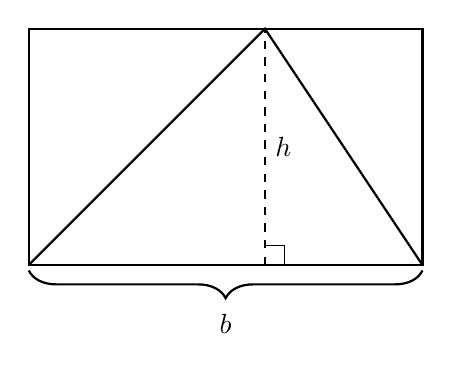
\begin{tikzpicture}
  % rectangle
  \draw[thick] (0,0) rectangle (5,3);
  % triangle
  \draw[thick] (0,0) -- (3,3) -- (5,0);
  % height
  \draw[thick,dashed] (3,0) -- node[midway, right] {\(h\)}(3,3);
  % right angle
  \draw (3.25,0) -- (3.25,0.25) -- (3,0.25);
  % brace to indicate length of base
  \draw[decorate,decoration={brace,amplitude=10pt,mirror, raise=2pt},thick]
  (0,0) -- node[midway,below,yshift=-0.5cm] {\(b\)} (5,0);
\end{tikzpicture}
\end{document}
